
\section{Training Curves}\label{sec:graphs:training_curves}

Both \textit{katz-eig} and \textit{link-analysis} are iterative algorithms. Their descriptions use the phrase "repeat until convergence".  With training curves, which plots the evaluation metric with the respect to epochs, the number of iterations, the effect of running more iterations can be seen.

The plots have recommendations calculated using the training set and evaluated against the training set for \textit{Precision}, \textit{Recall} and \textit{F-measure} using the top-10 recommendations. Each $K$ are different for each dataset, using a learned optimal value, and $beta = \frac{1}{\|A_{train}\|_2}$.

\subsection{katz-eig}

\FloatBarrier

\begin{figure}[h!]
\centering
\begin{minipage}{.5\textwidth}
    \centering
    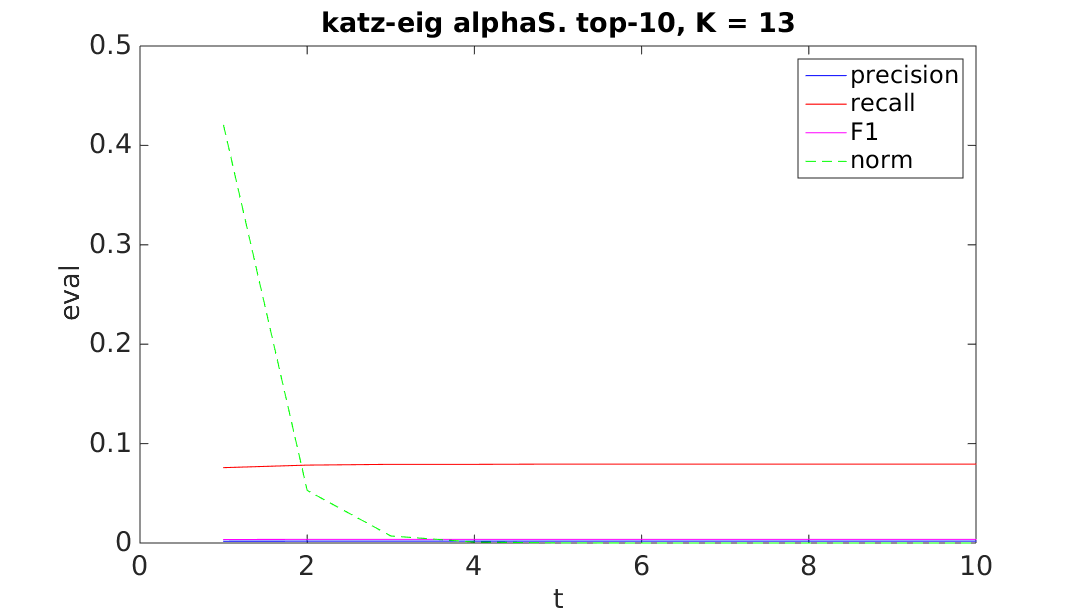
\includegraphics[width=\linewidth]{fig/katzeig_t/alphaS_katzeig_t.png}
    \captionof{figure}{\textit{alphaS}}
\end{minipage}%
\begin{minipage}{.5\textwidth}
    \centering
    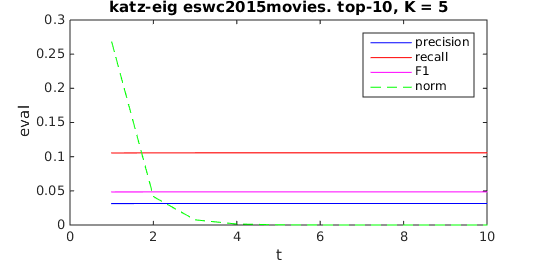
\includegraphics[width=\linewidth]{fig/katzeig_t/eswc2015movies_katzeig_t.png}
    \captionof{figure}{\textit{eswc2015movies}}
\end{minipage}
\end{figure}

\begin{figure}[h!]
\centering
\begin{minipage}{.5\textwidth}
    \centering
    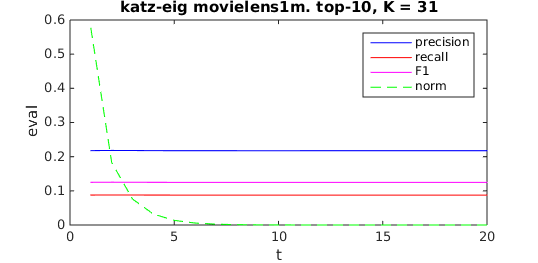
\includegraphics[width=\linewidth]{fig/katzeig_t/movielens_katzeig_t.png}
    \captionof{figure}{\textit{movielens1m}}
\end{minipage}%
\begin{minipage}{.5\textwidth}
    \centering
    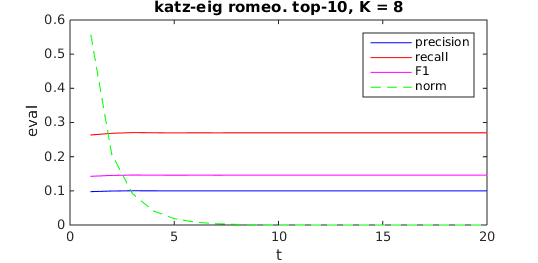
\includegraphics[width=\linewidth]{fig/katzeig_t/romeo_katzeig_t.png}
    \captionof{figure}{\textit{romeo}}
\end{minipage}
\end{figure}

\FloatBarrier

The jagged line represents $\|S_t - S_{t - 1}\|_2$, which is a measure of the difference between the current iteration $t$ and the previous iteration. This was made as a measure of the convergence criteria. Convergence was reached with relatively few iterations, but the matrix $S$ is small and the calculation has low complexity.

In all following usages of \textit{katz-eig}, a value of $\epsilon = 0.01$ was used to break iterations if $\|S_t - S_{t - 1}\|_2 < \epsilon$.

\newpage


\subsection{link-analysis}

\Warning[TODO]{ Finish this section! }

\textit{Similar analysis as for katz-eig}

\textit{link-analysis} had it's maximum number of iterations fixed as $t_{max} = 3$ for the remained of this thesis.


%\begin{itemize}
    %\item alphaS
    %\item eswc2015movies
    %\item eswc2015books (skip?)
    %\item movielens1m
    %\item romeo
%\end{itemize}


